\chapter[Aplicando Minería de Datos con RapidMiner]{Aplicando Minería de Datos con RapidMiner}
\label{ch:desmin}

\section{Identificación de datos y variables}
\subsection{Recolección de Datos}

Los datos a utilizar en los modelos a presentar en este capítulo son extraídos de la base de datos de la institución privada. Estos datos corresponde a información de los años 2014 y 2015 de alumnos de las distintas carreras de ingeniería que imparte la institución. Además se extrae información a través del SIES sobre la institución y sus diferentes carreras de ingeniería con respecto a acreditación e indices de empleabilidad.\\

Los datos proporcionados por la institución se encuentra en un archivo Excel en el cual figuran los siguientes datos: Rut del estudiante, Apellido paterno del estudiante, Apellido materno del estudiante, Nombres del estudiante, Comuna de residencia del estudiante, Ciudad de residencia del estudiante, Facultad del estudiante, Carrera del estudiante, Jornada del estudiante, PSU de lenguaje
PSU de matemáticas, PSU de ciencias, PSU de historia, Año de ingreso a la carrera, Código de la carrera, Semestre de inicio de la carrera, Notas de enseñanza media, Código RBD del colegio, Tipo de dependencia del colegio, Sexo del estudiante, Puntaje ranking del estudiante, Fecha de nacimiento del estudiante, Código de región del colegio, Región del colegio, Comuna del colegio, Nombre del colegio, Código del plan del alumno, Código del  plan de la carrera, Código del semestre de inicio de la carrera, Año de información, Semestre de información, Código del curso, Código del semestre de información, Semestre de ingreso a la carrera, Código del estado del curso inscrito, Código del estado del alumno al final del curso, Estado del alumno al final del curso, Sección del curso, Código del ramo, Nota final del curso, Ramo nemotecnico, Nombre del ramo, Nivel del ramo, Tipo de ramo, Código de semestre de inicio del plan (2014), Código de semestre de inicio de la carerra (2014), Sexo del estudiante, País gentilicio, Tipo de contrato, Correo personal, Teléfono fijo, Teléfono celular, Semestre de ingreso a la carrera, Código de la facultad, Beca fallecimiento (2014),Beca de cesantia (2014), Beca internado (2014), Beca Complementaria CAE (2014), Beca Mérito (2014), Beca de Almuerzo (2014), Beca de Fotocopia (2014), Beca de Plotter (2014), Beca Valech (2014), Beca Traspaso Valech (2014), Beca Indígena (2014), Beca Hijo de Profesor (2014), Beca Integración Territorial (2014), Beca Excelencia Mineduc (2014), Beca Juan Gómez Milla (2014), Beca Mun. de Las Condes (2014), Beca Puntaje Nacional (Interno) (2014), Beca Presidente de la Republica (2014), Beca Chaitén (2014), Beca Terremoto (2014), JUNAEB (2014), CAE (2014), Si tiene beca (2014), Si tiene beca interna (2014), Si tiene beca externa (2014), Beca Vocación de Profesor (2014), Mantención JUNAEB (2014), Beca Puntaje PSU MINEDUC (2014), Beca Deportista Destacado (2014), Beca Transporte (2014), Equidad (2014), Beca Complementaria Vocación de Profesor (2014), Beca de Honor (2014), Beca Balmaceda (2014), Beca Funcionario (2014), Beca Ranking NEM (2014),Beca Articulación (2014), Otra Beca MINEDUC (2014), Estado de plan alumno (2015), Código de semestre de inicio del plan (2015), Código de semestre de inicio de la carerra (2015), Beca fallecimiento (2015), Beca de cesantia (2015), Beca internado (2015), Beca Complementaria CAE (2015), Beca Mérito (2015), Beca de Almuerzo (2015), Beca de Fotocopia (2015), Beca de Plotter (2015), Beca Valech (2015), Beca Traspaso Valech (2015), Beca Indígena (2015), Beca Hijo de Profesor (2015), Beca Integración Territorial (2015), Beca Excelencia Mineduc (2015), Beca Juan Gómez Milla (2015), Beca Mun. de Las Condes (2015), Beca Puntaje Nacional (Interno) (2015), Beca Presidente de la Republica (2015), Beca Chaitén (2015), Beca Terremoto (2015), JUNAEB (2015), CAE (2015), Si tiene beca (2015), Si tiene beca interna (2015), Si tiene beca externa (2015), Beca Vocación de Profesor (2015), Mantención JUNAEB (2015), Beca Puntaje PSU MINEDUC (2015), Beca Deportista Destacado (2015), Beca Transporte (2015), Equidad (2015), Beca Complementaria Vocación de Profesor (2015), Beca de Honor (2015), Beca Balmaceda (2015), Beca Funcionario (2015), Beca Ranking NEM (2015), Beca Articulación (2015), Otra Beca MINEDUC (2015).

La información del SIES se encuentra en un sitio web, por lo que se creo una base de datos en MySQL llamada \textit{Area Staging} con toda la información recopilada.\\ 

\subsection{Procesamiento de Datos}

La información recopilada de las dos fuentes de datos fue procesada, extrayendo y transformando varios de los datos que se presentaron anteriormente. Este procesamiento se realizo a partir de las variables consideradas en los constructos y del análisis de diferentes investigaciones del tema deserción en Chile que indican que son buenos predictores del Capitulo \ref{ch:tema}.\\

\begin{figure}[H]
	\centering 
	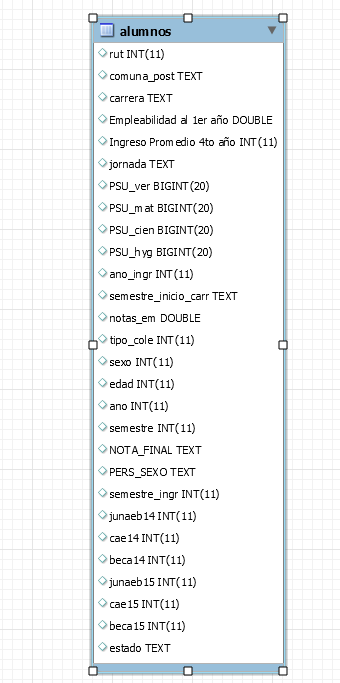
\includegraphics[width=8cm,height=8cm] {areastaging.png} 
	\caption[Tabla resultante]{Tabla resultante}
	\label{fig:bdarea}
\end{figure}

Los datos procesados se pueden apreciar en la Figura \ref{fig:bdarea}, la cual tiene principalmente variables de la ``Institución y Carrera'' y del ``Desempeño del Alumno'' definidas en el tablou de los constructos, Tabla \ref{tabla:Tablou de variables}, faltando las variables de ``Motivaciones del Alumno'', por lo que para efecto de este estudio, se propone un mecanismo para capturar estos datos.\\

El mecanismos a proponer es generar encuestas a final de cada semestre que capte y actualice las variables correspondientes a las motivaciones del alumno, de tal modo poder analizar la situación del alumno de manera semestral.\\

\subsection{Muestra de Datos}

La muestra de datos esta configurada para dos conjuntos de datos, el primero lo conforma datos de alumnos de jornada diurna y el segundo conjunto por alumnos de jornada vespertina.\\

El conjunto de alumnos de jornada diurna esta conformado por 709 observaciones, de los cuales 11 representan abandono.\\

El conjunto de alumnos de jornada vespertina esta conformado por 49 observaciones, de los cuales dos representan abandono.\\

\subsection{Variables}

A continuación se muestra una tabla con variable para modelar los datos de los dos conjuntos, el conjunto de jornada de vespertina no se consideran los puntajes PSU debido a que la institución tiene otro mecanismo de ingreso y la mayoría de las observaciones tiene esos campos vacíos.\\

\begin{longtable}{| p{3cm}| p{2cm} | p{7cm} |}
			\hline
			Variable & Tipo & Descripción \\
			\hline \hline
			\endfirsthead
			
			\hline
            Variable & Tipo & Descripción \\
            \hline \hline
            \endhead
            Rut & N/A & Identificador	\\ \hline			
			Comuna & N/A & Nombre de las comunas de residencia\\ \hline
			Genero & Discreto & Toma los siguientes valores, Femenino = 1; Masculino=2; F=1\\ \hline
			Edad & Continuo & Se considera edad del año 2014\\ \hline
			Tipo establecimiento de origen & Discreto & Toma los siguientes valores, Municipal=1; Particular Subvencionado=2; Particular Pagado =3;\\ \hline
			Notas enseñanza media & Continuo & Rango entre 10 y 70\\ \hline
			PSU lenguaje matemáticas & Continuo & Rango de 150 a 850\\ \hline
			PSU matemáticas & Continuo & Rango de 150 a 850\\ \hline
			PSU ciencias & Continuo & Rango de 150 a 850\\ \hline				
			Acreditación Institucional & Discreto & Toma los siguientes valores,  No Acreditada=0; Acreditada=1\\ \hline
			Carrera & N/A & Nombre de carrera\\ \hline
			Jornada & Discreto & Toma los siguientes valores,  Diurna y Vespertina\\ \hline
			Empleabilidad al 1er año & Continuo & Rango en porcentaje 0 a 100\\ \hline
			Ingreso promedio 4to año & Continuo & Rango en dinero\\ \hline
			Carrera acreditada & Discreto & Toma los siguientes valores,  No Acreditada=0; Acreditado=1\\ \hline 
			Promedio notas acumuladas & Continuo & Rango entre 10 y 70 \\ \hline
			Beca14 & Discreto & Toma los siguientes valores,  No Beca=0; beca=1\\ \hline
			Beca15 & Discreto & Toma los siguientes valores,  No Beca=0; beca=1\\ \hline
			Junaeb14 & Discreto & Toma los siguientes valores,  No Junaeb=0; Junaeb=1\\ \hline
			Junaeb15 & Discreto & Toma los siguientes valores,  No Junaeb=0; Junaeb=1\\ \hline
			Cae14 & Discreto  & Toma los siguientes valores,  No Cae=0; Cae=1 \\ \hline
			Cae15 & Discreto & Toma los siguientes valores,  No Cae=0; Cae=1\\ \hline
			Estado & Discreto & Toma los siguientes valores,  Activo y Abandono\\ \hline
			 \hline
		\caption{Variables.}
		\label{tabla:variablesdiurna}
\end{longtable}	



En las tablas anteriormente presentadas, se definió dos tipos de variables \cite{variables}:

\begin{itemize}
	\item Variables Discretas: Son variables que toma un conjunto de valores determinados, es decir, no acepta cualquier valor, solo los que existen el en conjunto, por ejemplo, Genero toma dos valores, Masculino y Femenino.
	\item Variables Continuas: Son variables que pueden tomar un valor fijo dentro de un intervalo, por ejemplo, los puntajes PSU puede tomar cualquier valor dentro del rango 150 a 850.
\end{itemize} 





\subsection{Procesos en RapidMiner}

La construcción de los modelos se implementará con la herramienta \textit{RapidMiner} utilizando como entrada las tablas generadas anteriormente.\\

\begin{figure}[H]
	\centering 
	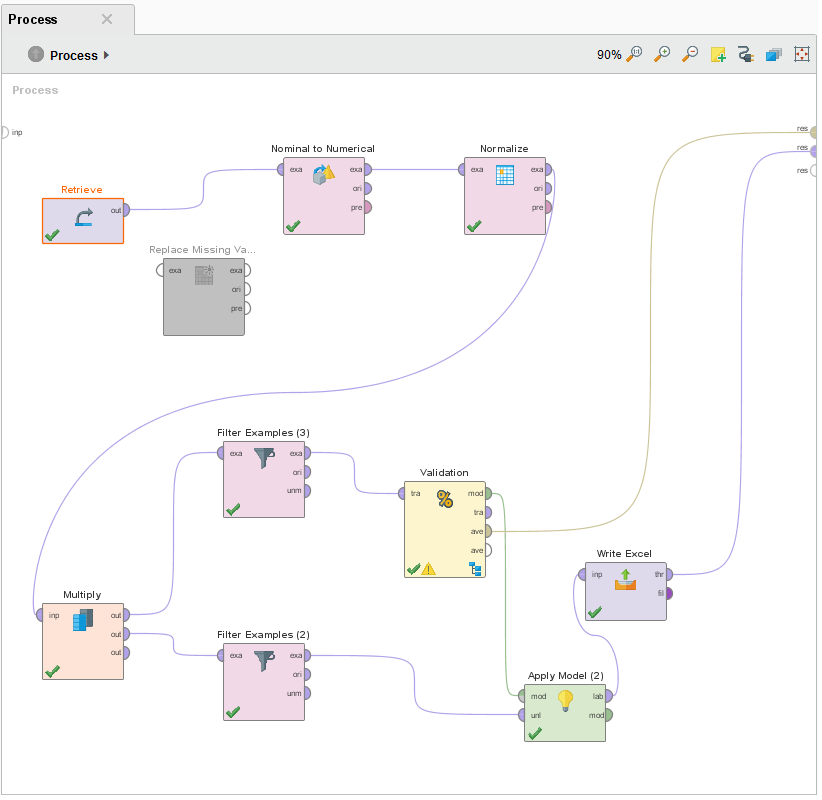
\includegraphics[width=12cm,height=7cm] {proceso.png} 
	\caption[Proceso de Predicción]{Proceso de Predicción}
	\label{fig:proceso}
\end{figure}

La herramienta \textit{RapidMiner} permite a través de operadores, construir un proceso. Los procesos son una serie de pasos constituidos por operadores. La Figura \ref{fig:proceso} representa el proceso construido para generar la predicción de los datos. La descripcion de cada operador se detalla en el Anexo \ref{ch:anexo-b}\\
 

\begin{figure}[H]
	\centering 
	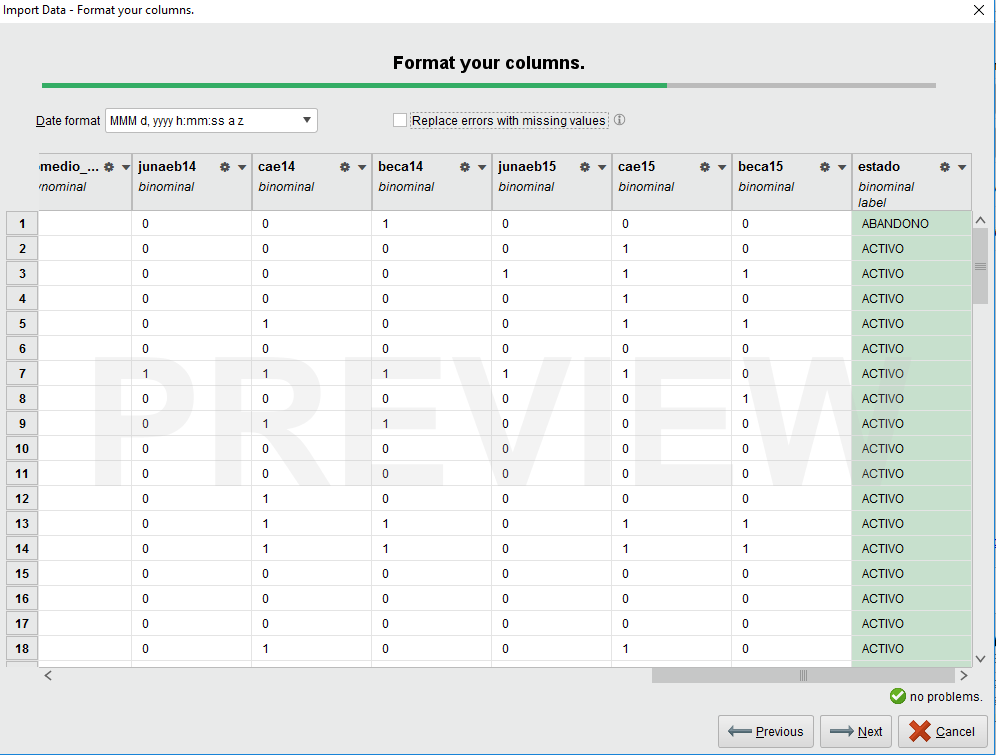
\includegraphics[width=12cm,height=7cm] {importdatos.png} 
	\caption[Importación de datos]{Importación de datos}
	\label{fig:importdata}
\end{figure}

El primer paso antes de operar el proceso construido, es importar los datos para entrenar y predecir. Las variables se definen con el tipo de dato que las caracteriza junto al rol a cumplir dentro del modelo, para este caso, se tomo como rol identificador la variable ``rut'' y como variable a predecir ``estado'', Figura \ref{fig:importdata}.

\begin{figure}[H]
	\centering 
	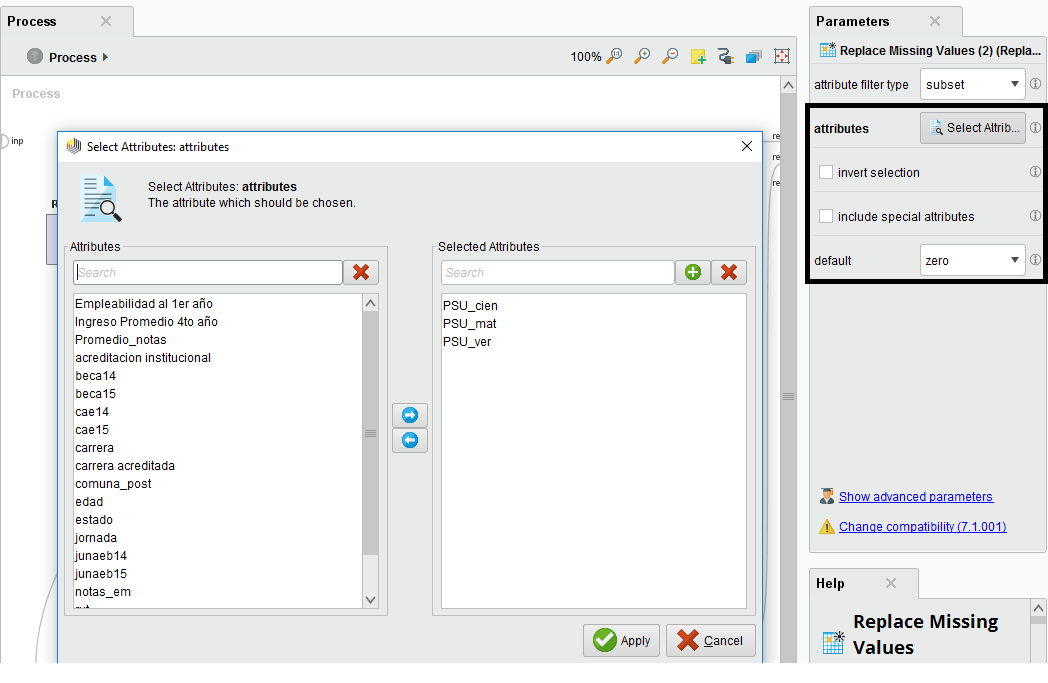
\includegraphics[width=12cm,height=7cm] {remplazodatos.png} 
	\caption[Remplazar de datos vacios]{Remplazar de datos vacíos}
	\label{fig:remplazadata}
\end{figure}

Los datos cargados son accedidos por el operador ``Retrieve'' y luego pasados hacia el operador ``Replace Missing Values'' el cual reemplaza los valores vacíos de las variables seleccionadas, en este caso se seleccionaron las variables de ``PSU'' los cuales tienen datos vacíos, estos datos serán reemplazados por ceros como se puede ver en la Figura \ref{fig:remplazadata}.\\

Luego de que los datos son reemplazados, pasan al operador ``Nominal to Numerical'', el cual transforma todas la variables a numéricas, para luego pasar al operador ``Normalize'', normalizando los datos y luego al operador ``Multiply'' el cual multiplica los datos generando dos conjuntos, el primero para ser entrenado y el otro para validar, separados por los operadores ``Filter Example''.\\


\begin{figure}[H]
	\centering 
	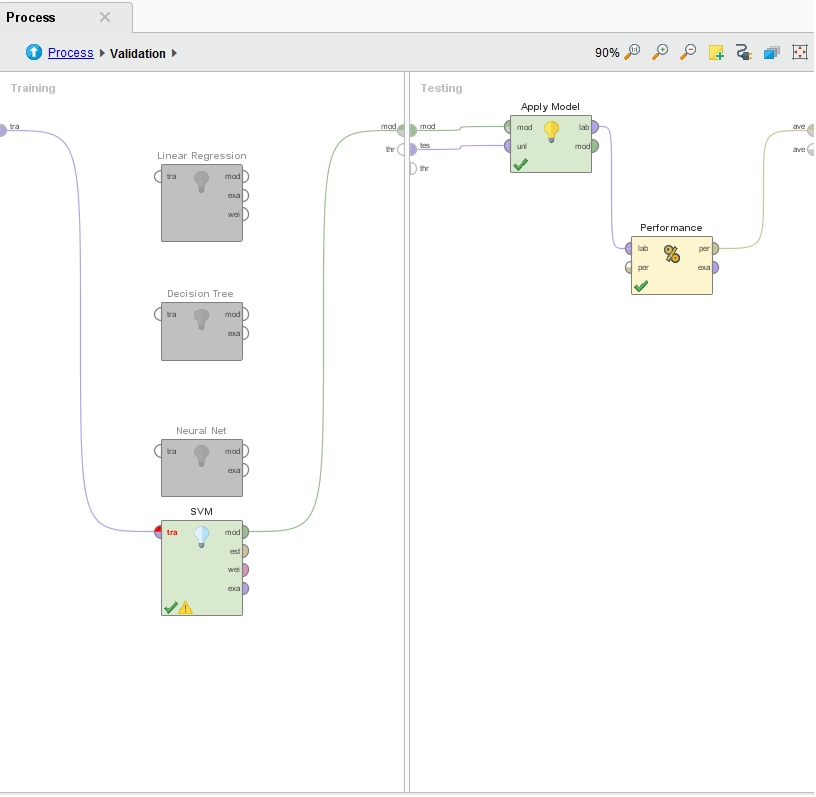
\includegraphics[width=12cm,height=7cm] {provalidacion.png} 
	\caption[Validación]{Validación}
	\label{fig:validacion}
\end{figure}

En el operador ``Validation'' se definen el porcentaje de datos a entrenar del total del conjunto de datos, en este caso se especifica un 70 \%. En este operador, se puede seleccionar los operadores de predicción, que para este estudio serán los cuatros que se muestran en la Figura \ref{fig:validacion}.

\section{Modelamiento}

El modelamiento se configuro de la siguiente manera, para el conjunto de datos de jornada diurna, se replicaron 53 observaciones dejando la variable a predecir vacía. Y para el conjunto de datos de jornada vespertina, se replicaron 21 observaciones dejando la variable a predecir vacía.\\

El detalle del resultado de las cuatro técnicas de predicción utilizadas en los conjuntos de datos, se especifica la matriz de confusión, las variables que más influyeron en cada predicción y el porcentaje real de predicción.\\

La matriz de confusión es una herramienta que permite visualizar el desempeño de un algoritmo empleado para aprendizaje supervisado. Las columnas representan el número de predicciones por clases y las filas representan las instancias de la clase. Esta herramienta permite ver si el sistema esta confundiendo dos clases \cite{matriz}.\\


\subsection{SVN}

\begin{itemize}
	\item Jornada Diurna\\
	
\begin{figure}[H]
	\centering 
	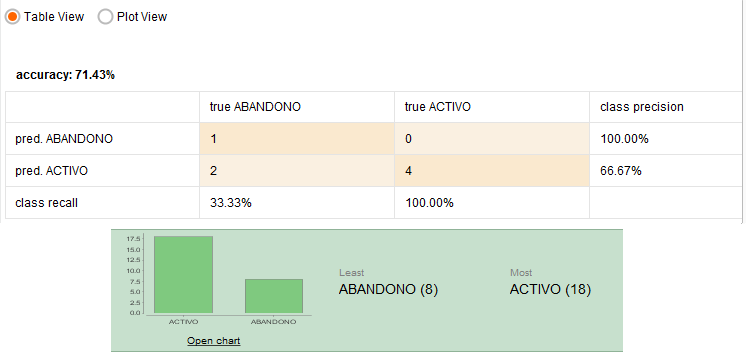
\includegraphics[width=10cm,height=3cm] {svndiurno.png} 
	\caption[Matriz de Confusión SVN Diurno]{Matriz de Confusión SVN Diurno}
	\label{fig:svndiurno}
\end{figure}	
	
La matriz de confusión que se muestra en la Figura \ref{fig:svndiurno} indica que SVN obtuvo una precisión del 98.12\%, especificando que la clase ACTIVO tuvo una precisión del 99.52\%, mientras que la clase ABANDONO tuvo 0\%. Sin embargo comparando las observaciones predichas con las observaciones reales, se obtuvo una precisión del 100\%.

Las variables con mayor peso en la predicción de la clase ACTIVO fueron: CAE15, PSU Ciencias, Beca15, Promedio notas, Carrera, Empleabilidad al 1er año, Junaeb15, NEM, Ingreso Promedio 4to año, Tipo colegio, Comuna y Genero.\\



\item Jornada Vespertina\\	

\begin{figure}[H]
	\centering 
	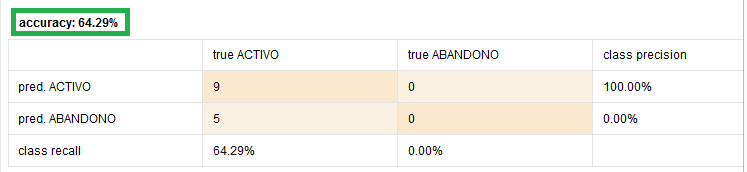
\includegraphics[width=10cm,height=3cm] {svnvesp.png} 
	\caption[Matriz de Confusión SVN Vespertino]{Matriz de Confusión SVN Vespertino}
	\label{fig:svnvesp}
\end{figure}	

La matriz de confusión que se muestra en la Figura \ref{fig:svnvesp} indica que SVN obtuvo una precisión del 64.29\%, especificando que la clase ACTIVO tuvo una precisión del 100\%, mientras que la clase ABANDONO tuvo 0\%. Sin embargo comparando las observaciones predichas con las observaciones reales, se obtuvo una precisión del 100\%.

Las variables con mayor peso en la predicción de la clase ACTIVO fueron: Edad, NEM, Genero, Comuna, Junaeb14 y Junaeb15.\\

				
	
\end{itemize}

\subsection{Regresión Lineal}

\begin{itemize}
	\item Jornada Diurna\\
	
	\begin{figure}[H]
		\centering 
		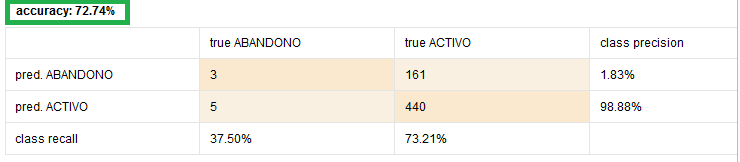
\includegraphics[width=10cm,height=3cm] {rldiurno.png} 
		\caption[Matriz de Confusión Regresión Lineal Diurno]{Matriz de Confusión Regresión Lineal Diurno}
		\label{fig:rldiurno}
	\end{figure}	
	
	La matriz de confusión que se muestra en la Figura \ref{fig:rldiurno} indica que Regresión Lineal obtuvo una precisión del 72.74\%, especificando que la clase ACTIVO tuvo una precisión del 98.88\%, mientras que la clase ABANDONO tuvo 1.83\%. Sin embargo comparando las observaciones predichas con las observaciones reales, se obtuvo una precisión del 81.13\%.
	
	 Las variables con mayor peso en la predicción de la clase ACTIVO fueron: NEM, CAE15, PSU Ciencias, Tipo colegio, Junaeb14, Promedio notas, Comuna y Edad.\\
	

	
	\item Jornada Vespertina\\	
	
\begin{figure}[H]
	\centering 
	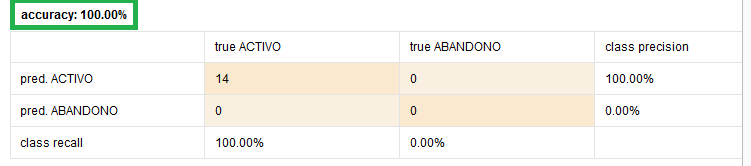
\includegraphics[width=10cm,height=3cm] {rlvesp.png} 
	\caption[Matriz de Confusión Regresión Lineal Vespertino]{Matriz de Confusión Regresión Lineal Vespertino}
	\label{fig:rlvesp}
\end{figure}	

La matriz de confusión que se muestra en la Figura \ref{fig:svnvesp} indica que Regresión Lineal obtuvo una precisión del 100\%, especificando que la clase ACTIVO tuvo una precisión del 100\%, mientras que la clase ABANDONO tuvo 0\%. Sin embargo comparando las observaciones predichas con las observaciones reales, se obtuvo una precisión del 95.23\%.

Las variables con mayor peso en la predicción de la clase ACTIVO fueron: CAE14, Comuna y Beca15.\\

	
\end{itemize}


\subsection{Red Neuronal}

\begin{itemize}
	\item Jornada Diurna\\
	
	\begin{figure}[H]
		\centering 
		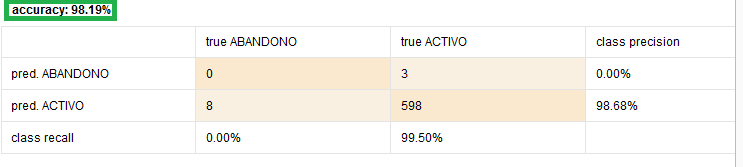
\includegraphics[width=10cm,height=3cm] {rndiurno.png} 
		\caption[Matriz de Confusión Red Neuronal Diurno]{Matriz de Confusión Red Neuronal Diurno}
		\label{fig:rndiurno}
	\end{figure}	
	
	La matriz de confusión que se muestra en la Figura \ref{fig:rndiurno} indica que Red Neuronal obtuvo una precisión del 98.19\%, especificando que la clase ACTIVO tuvo una precisión del 98.68\%, mientras que la clase ABANDONO tuvo 0\%. Sin embargo comparando las observaciones predichas con las observaciones reales, se obtuvo una precisión del 94.34\%.
	
	Se genero 127 nodos en donde las variables con mayor peso en la predicción de la clase ACTIVO fueron: NEM, Comuna y Edad.\\

	
	
	\item Jornada Vespertina\\	
\begin{figure}[H]
	\centering 
	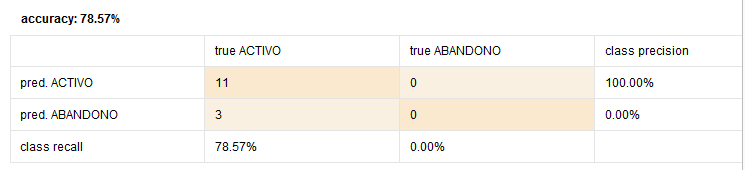
\includegraphics[width=10cm,height=3cm] {rnvesp.png} 
	\caption[Matriz de Confusión Red Neuronal Vespertino]{Matriz de Confusión Red Neuronal Vespertino}
	\label{fig:rnvesp}
\end{figure}	

La matriz de confusión que se muestra en la Figura \ref{fig:rnvesp} indica que Red Neuronal obtuvo una precisión del 78.57\%, especificando que la clase ACTIVO tuvo una precisión del 100\%, mientras que la clase ABANDONO tuvo 0\%. Sin embargo comparando las observaciones predichas con las observaciones reales, se obtuvo una precisión del 100\%.

Se genero 22 nodos en donde las variables con mayor peso en la predicción de la clase ACTIVO fueron: tipo de colegio, Comuna, Promedio notas, Junaeb14, CAE14, Beca14, Junaeb15, CAE15 y Beca15.\\


	
\end{itemize}

\subsection{Árbol de Decisión}

\begin{itemize}
	\item Jornada Diurna\\
	
	\begin{figure}[H]
		\centering 
		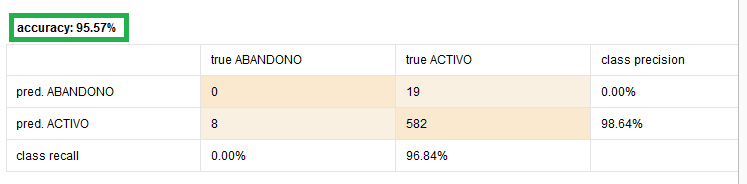
\includegraphics[width=10cm,height=3cm] {addiurna.png} 
		\caption[Matriz de Confusión]{Matriz de Confusión}
		\label{fig:addiurna}
	\end{figure}	
	
	La matriz de confusión que se muestra en la Figura \ref{fig:addiurna} indica que Árbol de Decisión obtuvo una precisión del 95.57\%, especificando que la clase ACTIVO tuvo una precisión del 98.64\%, mientras que la clase ABANDONO tuvo 0\%. Sin embargo comparando las observaciones predichas con las observaciones reales, se obtuvo una precisión del 81.13\%.
	
	La variable con mayor peso en la predicción de la clase ACTIVO fue: Comuna.\\
	

	
	\item Jornada Vespertina\\	
	
		\begin{figure}[H]
		\centering 
		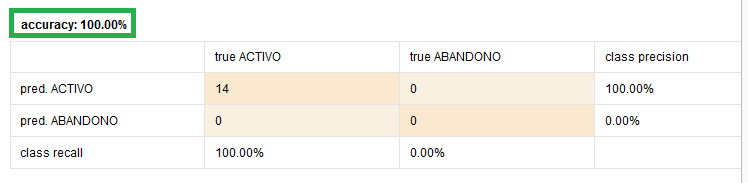
\includegraphics[width=10cm,height=3cm] {advesp.png} 
		\caption[Matriz de Confusión]{Matriz de Confusión}
		\label{fig:advesp}
	\end{figure}	
	
	La matriz de confusión que se muestra en la Figura \ref{fig:advesp} indica que Árbol de Decisión obtuvo una precisión del 100\%, especificando que la clase ACTIVO tuvo una precisión del 100\%, mientras que la clase ABANDONO tuvo 0\%. Sin embargo comparando las observaciones predichas con las observaciones reales, se obtuvo una precisión del 90.48\%.
	
		La variable con mayor peso en la predicción de la clase ACTIVO fue: Promedio de notas.\\
	
	 
		
\end{itemize}

En ambos casos de los conjuntos probados en los cuatro algoritmos utilizados, las matrices de confusión tienen un sesgo hacia la predicción ACTIVO, por lo que en todos los casos se realizo una comparación de las observaciones a predecir con las observaciones que tienen definido su estado.\\

\section{Resultados}

